\documentclass{article}[18pt]
\usepackage{../../../../format}
\lhead{Theory of Computation - Algorithms and Complexity}
\lstset{language=C,
	basicstyle=\ttfamily,
	keywordstyle=\bfseries,
	showstringspaces=false,
	morekeywords={if, else, then, print, end, for, do, while},
	tabsize=4,
	mathescape=true,
	escapechar=£,
	numbers=left,
	stepnumber=1,
}

\usepackage{caption}
\DeclareCaptionFont{white}{\color{white}}
\DeclareCaptionFormat{listing}{\colorbox{gray}{\parbox{\textwidth}{#1#2#3}}}
\captionsetup[lstlisting]{format=listing,labelfont=white,textfont=white}

\begin{document}
\begin{center}
\underline{\huge Dynamic Programming I - Rod Cutting}
\end{center}
\section{Rod cutting problem}
You work for a company that buys steel rods and cuts them into shorter rods, which it then sells.\\
\\
You are asked to determine the best way to cut the rods to maximise profit.\\
\\
You know, for $i=1,...,n$, the price $p_i$ in euros that the company charges for a rod of length $i$ centimetres (Rod lengths are always an integer number of centimetres)\\
\\
E.g.
\begin{center}
	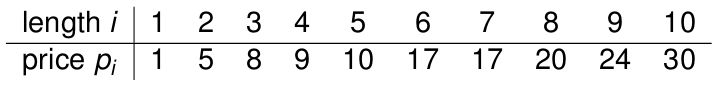
\includegraphics[scale=0.7]{Rod}
\end{center}
\subsection{More formally}
\begin{defin}[Rod cutting problem]
Given a rod of length n and a table of prices $p_i$ for $i=1,...,n$, determine the maximum revenue $r_n$ obtained by cutting up the rod and selling the pieces
\end{defin}
E.g. with $n=4$ and $p_1=1, p_2=5, p_3=8, p_4=9$\\
\\
By brute force: list all possible ways of cutting up $n=4$
\[
\begin{array}{c|c|c|c|c|c|c}{\text { Partition }} & {4} & {1+3} & {2+2} & {1+1+2} & {1+1+1+1} \\ \hline \text { Revenue } & {9} & {9} & {10} & {7} & {4}\end{array}
\]
Maximum revenue if we cut two rods of length 2, and we have $r_4=10$
\subsection{A note on integer partitions}
\begin{defin}[Integer partition]
An integer partition of a positive integer n is a list of positive integers $\langle a_1,...,a_k \rangle$ such that $a_1\leqslant a_2\leqslant ... \leqslant a_k$ and
\[
\sum_{i=1}^{k} a_{i}=n
\]	
\end{defin}
Let $p(n)$ denote the number of integer partitions of n, then
$$p(1)=2, p(2)=2, p(3)=3, p(4)=5...$$
Hardy and Ramanujan proved that
\[
p(n) \sim \frac{1}{4 n \sqrt{3}} \exp (\pi \sqrt{\frac{2 n}{3}})
\]
Therefore, brute force has an exponential running time
\section{Dynamic Programming}
\subsection{Optimal substructure}
More generally, we have for all $n\geqslant 1$
\[
r_{n}=\max \left\{p_{i}+r_{n-i}: 1 \leq i \leq n\right\}
\]
Idea: $p_n$ corresponds to no cuts and $p_i+r_{n-i}$ to cutting into a rod of length $i$ and another rod of length $n-i$\\
\\
To solve the original problem of size n, we solve independent smaller problems of the same type, but of smaller sizes
\begin{defin}[Optimal substructure]
Optimal solutions to a problem incorporate optimal solutions to related subproblems, which we may solve independently	
\end{defin}
\subsection{Recursive top-down implementation}
Input: an array $p[1..n]$ of prices and an integer n\\
\\ 
Output: The maximum revenue possible for a rod of length n
\begin{lstlisting}[caption=ROD({p,n})]
if n==0 then
	return 0
q $\leftarrow$ -1
for i $\leftarrow$ 1 to n do
	q=max{q,p[i]+ROD(p,n-i)}
return q
\end{lstlisting}
The running time for this is exponential again (there are $2^n$ calls of the form ROD(p,k) for $n\geqslant 1$)
\subsection{Using dynamic programming for optimal rod cutting}
The naive recursion solution is slow because it repeatedly solves the same subproblems\\
\\
We arrange the subproblems in order to solve them only one, saving its solution. If we need that solution, we just look it up: we needn't recompute it\\
\\
Dynamic programming thus uses additional memory to save computation: it is an example of time-memory trade-off\\
\\
A dynamic programming approach runs in polynomial time when the number of distinct subproblems involved is polynomial and we can solve each subproblem in polynomial time
\subsection{Overlapping subproblems}
In the naive top-down method, we keep on solving the same subproblems: we say that these subproblems overlap. Memoization prevents that. Careful
\begin{itemize}
	\item Two subproblems are independent if they do not share resources
	\item Two subproblems are overlapping if they are really the same subproblem that occurs as a subproblem of different problems
\end{itemize}
\section{Top-down vs Bottom-up}
First approach: top-down with memoization\\
\\
We write the procedure recursively in a natural manner, but modified to save the result of each subproblem (usually in an array)\\
\\
The procedure checks if it has previously solved this subproblem; if not, the procedure computes the value in the usual manner\\
\\
We say the recursive procedure has been memoized: it remembers what results it has computed previously.
\subsection{Rod cutting: Top-down with memoization}
\begin{lstlisting}[caption=MEMOIZED-ROD({p,n})]
Let r[0..n] be a new array
for i $\leftarrow$ 0 to n do
	r[i] $\leftarrow$ -1
return MEMOIZED-ROD-AUX(p,n,r)
\end{lstlisting}

\begin{lstlisting}[caption=MEMOIZED-ROD-AUX({p,n,r})]
if r[n]$\geqslant$ 0 then
	return r[n]
if n==0 then
	q $\leftarrow$ 0
else
	q $\leftarrow$ -1
	for i $\leftarrow$ 1 to n do
		q $\leftarrow$ max{q,p[i]+MEMOIZED-ROD-AUX(p,n-i,r)}
r[n] $\leftarrow$ q
return q
\end{lstlisting}
\subsection{Second approach}
Second approach to implement dynamic programming: Bottom-up method\\
\\
It depends on the idea of the "size" of a subproblem, such that solving any particular subproblem relies on solving smaller subproblems\\
\\
We sort the subproblems by size and solve them in size order, smallest first. We save the solutions.\\
\\
We solve each subproblem only once, and when we first see it, we have solved all its prerequisite subproblems.
\begin{lstlisting}[caption=BOTTOM-UP-ROD({p,n})]
Let r[0..n] be a new array
r[0] $\leftarrow$ 0
for j $\leftarrow$ 1 to n do
	q $\leftarrow$ -1
	for i $\leftarrow$ 1 to j do
		q $\leftarrow$ max{q,p[i]+r[j-i]}
	r[j]$\leqslant$ q
return r[n]
\end{lstlisting}
\subsection{Running time}
For rod cutting, both approaches have a worst case running time of $\Theta(n^2)$\\
\\
Easy to see for bottom-up\\
\\
The memoized approach solves each subproblem for sizes 0,1,...,n once. To solve a problem of size n, the for loop iterates n times. The total number of iterations is an arithmetic series.\\
\\
Usually, both approaches have the same complexity, but the bottom-up approach has lower constants, due to less overhead for procedure calls


\end{document}